\documentclass[12pt,a4paper]{ctexart}

% ==================== 页面设置 ====================
\usepackage[top=2.5cm, bottom=2.5cm, left=2.5cm, right=2.5cm]{geometry}
\usepackage{graphicx}
\usepackage{booktabs}
\usepackage{amsmath}
\usepackage{amssymb}
\usepackage{hyperref}
\usepackage{caption}
\usepackage{subcaption}
\usepackage{float}
\usepackage{enumitem}
\usepackage{xcolor}
\usepackage{multirow}
\usepackage{array}
\usepackage{listings}

\hypersetup{
    colorlinks=true,
    linkcolor=blue,
    urlcolor=blue,
    citecolor=blue
}

% ==================== 标题 ====================
\title{\textbf{皮肤镜图像分类中的增强数据鲁棒性测试与稳定性分析}}
\author{成员4：鲁棒性测试、结果对比与指标分析模块}
\date{\today}

\begin{document}

\maketitle

\begin{abstract}
本报告针对皮肤镜图像三分类任务（黑色素瘤 mel、痣 nv、血管病变 vasc），在成员1完成图像预处理与数据集划分、成员2完成127维颜色纹理特征提取、成员3完成传统机器学习模型训练与基础评估的基础上，进一步开展增强数据鲁棒性测试、结果对比和稳定性分析。实验围绕SVM、随机森林（Random Forest）和K近邻（KNN）三种传统模型展开，首先复现成员3在干净测试集上的基线性能，然后从三个角度检验模型稳定性：一是分析增强图像在测试集中的预测一致性；二是对测试图像施加亮度、对比度、高斯噪声、模糊、旋转裁剪等扰动并重新提取特征；三是按原始图像编号进行严格分组划分，避免同一原图的增强版本同时出现在训练集和测试集。实验结果表明，原始划分中训练集与测试集存在98个原始编号重叠，增强版本跨集合分布会使评估结果偏乐观；在严格分组划分下，随机森林的Macro-F1为0.5783$\pm$0.0346，SVM为0.5145$\pm$0.0496，KNN为0.4903$\pm$0.0671。扰动实验中，高斯噪声和亮度变化对模型影响最明显，其中SVM在高斯噪声$\sigma=16$条件下Macro-F1降至0.2026。综合来看，随机森林在严格分组和多数扰动下表现更稳定，SVM在干净测试集上对少数类覆盖较好，KNN对划分变化和扰动更敏感。
\end{abstract}

% ==================== 1. 引言 ====================
\section{引言}

\subsection{任务背景}
本模块是 ``Project 2：皮肤镜图像分类'' 大作业的第四部分。成员3已经基于成员2输出的127维手工特征完成了SVM、随机森林和KNN三种传统模型的训练、调参和测试集评估。然而，基础测试集指标只能说明模型在当前划分下的性能，并不能充分回答模型在增强图像、图像质量变化以及更严格数据划分条件下是否稳定。

因此，本模块重点关注模型鲁棒性与稳定性。对于医学图像分类任务而言，图像亮度、对比度、噪声、轻微模糊或拍摄角度变化都可能影响特征分布；同时，如果同一原始图像的增强版本同时出现在训练集和测试集，测试结果可能偏乐观。成员4的任务正是补充这一层分析，为最终项目报告提供更可信的模型选择依据。

\subsection{任务目标}
\begin{enumerate}[label=(\arabic*)]
    \item 复现成员3在干净测试集上的SVM、随机森林和KNN基线指标；
    \item 分析增强图像的预测一致性，统计原图与增强图在训练集和测试集之间的重叠风险；
    \item 对测试图像施加亮度、对比度、高斯噪声、模糊、旋转裁剪五类扰动，比较三种模型的性能下降；
    \item 按原始编号进行严格分组划分，避免同源增强图像泄漏，并进行10次随机稳定性测试；
    \item 输出Accuracy、Precision、Recall、Macro-F1、Weighted-F1、各类别F1、预测不变率、性能保持率和混淆矩阵等指标。
\end{enumerate}

\subsection{数据与输入文件}
本模块使用成员1--3已经生成的文件作为输入：
\begin{itemize}
    \item 图像数据：\texttt{train/} 480张图像，\texttt{test/} 120张图像；
    \item 标签文件：\texttt{train\_label.csv} 与 \texttt{test\_label.csv}；
    \item 特征文件：\texttt{features/X\_train\_norm.npy}、\texttt{features/X\_test\_norm.npy} 等127维标准化特征；
    \item 成员3结果：\texttt{results/evaluation\_results.pkl}、\texttt{results/model\_comparison.csv} 等模型与评估结果。
\end{itemize}

类别分布为：训练集 mel: 168，nv: 240，vasc: 72；测试集 mel: 42，nv: 60，vasc: 18。三类标签分别表示黑色素瘤、痣和血管病变。

% ==================== 2. 方法 ====================
\section{鲁棒性测试方法}

\subsection{基线复现}
首先加载成员2输出的标准化测试特征 \texttt{X\_test\_norm.npy} 和成员3保存的最优模型，对SVM、随机森林、KNN分别计算干净测试集上的指标。该结果作为所有扰动和严格分组实验的baseline。

对于每个模型 $f$，干净测试集预测为：
\begin{equation}
    \hat{y}_{clean} = f(X_{test})
\end{equation}
后续扰动条件下的结果均与该baseline进行对比。

\subsection{增强一致性分析}
数据集中每张原始图像可能存在 \texttt{\_aug1}、\texttt{\_aug2} 等增强版本。本模块将 \texttt{image\_id} 去除增强后缀后得到原始编号：
\begin{equation}
    id_{base} = \text{remove\_suffix}(id, \{\text{\_aug1}, \text{\_aug2}\})
\end{equation}

对测试集中同一原始编号下的多个样本，计算预测一致率：
\begin{equation}
    Consistency = \frac{1}{G} \sum_{g=1}^{G} \mathbb{I}\left(\left|\{\hat{y}_i: i \in g\}\right| = 1\right)
\end{equation}
其中 $G$ 表示测试集中包含至少两个增强版本的原始编号组数。

\subsection{扰动鲁棒性测试}
为了模拟真实应用中可能出现的图像质量变化，本模块对测试图像施加五类扰动，并重新提取与成员2一致的127维特征：
\begin{table}[H]
\centering
\caption{扰动鲁棒性测试设置}
\label{tab:perturb_settings}
\begin{tabular}{lll}
\toprule
\textbf{扰动类型} & \textbf{强度设置} & \textbf{含义} \\
\midrule
亮度变化 & factor=0.80, 1.20 & 模拟偏暗或偏亮图像 \\
对比度变化 & factor=0.80, 1.20 & 模拟成像对比度变化 \\
高斯噪声 & $\sigma$=8, 16 & 模拟传感器噪声或压缩噪声 \\
模糊 & radius=1, 2 & 模拟轻微失焦或运动模糊 \\
旋转裁剪 & 5$^\circ$/0.96, 10$^\circ$/0.92 & 模拟拍摄角度变化与边缘裁剪 \\
\bottomrule
\end{tabular}
\end{table}

每种扰动后使用成员2保存的 \texttt{StandardScaler} 进行标准化，再输入成员3训练好的模型。扰动条件下的性能保持率定义为：
\begin{equation}
    Retention_{F1} = \frac{F1_{perturbed}}{F1_{clean}}
\end{equation}
预测不变率定义为：
\begin{equation}
    Invariance = \frac{1}{N}\sum_{i=1}^{N}\mathbb{I}(\hat{y}_{i,perturbed}=\hat{y}_{i,clean})
\end{equation}

\subsection{严格分组稳定性测试}
原数据划分是以增强后的样本为单位划分的，因此可能出现同一原始图像的不同增强版本分别落入训练集和测试集。为了检验更真实的泛化性能，本模块将同一原始编号下的原图和增强图全部放在同一侧，再进行分层随机划分。

具体流程如下：
\begin{enumerate}[label=(\arabic*)]
    \item 合并原训练集和测试集的600个增强后样本；
    \item 根据去除 \texttt{\_aug1}/\texttt{\_aug2} 后的原始编号建立分组；
    \item 按原始编号进行80/20分层随机划分，确保同一组不跨训练集和测试集；
    \item 使用成员3确定的最优超参数重新训练SVM、随机森林和KNN；
    \item 重复10个随机种子，报告均值和标准差。
\end{enumerate}

\subsection{评价指标}
本模块沿用成员3的分类指标，并额外加入稳定性指标：
\begin{itemize}
    \item \textbf{Accuracy}：整体预测正确比例；
    \item \textbf{Precision / Recall / F1-score}：按类别计算精确率、召回率和F1；
    \item \textbf{Macro-F1}：三类F1的算术平均，对少数类更敏感；
    \item \textbf{Weighted-F1}：按类别样本量加权后的F1；
    \item \textbf{Prediction Invariance}：扰动前后预测标签保持不变的比例；
    \item \textbf{F1 Retention}：扰动后Macro-F1相对干净测试集Macro-F1的保持比例。
\end{itemize}

% ==================== 3. 实验设置 ====================
\section{实验设置}

\subsection{模型配置}
本模块不重新进行大规模网格搜索，而是使用成员3已经确定的最优模型配置：
\begin{table}[H]
\centering
\caption{成员4鲁棒性实验使用的模型参数}
\label{tab:model_params}
\begin{tabular}{lll}
\toprule
\textbf{模型} & \textbf{关键参数} & \textbf{说明} \\
\midrule
SVM & C=100, kernel=rbf, gamma=scale & 成员3推荐模型，概率输出开启 \\
Random Forest & n\_estimators=100, max\_depth=None & 成员3调优得到的随机森林配置 \\
KNN & n\_neighbors=1, weights=distance, metric=manhattan & 成员3调优得到的KNN配置 \\
\bottomrule
\end{tabular}
\end{table}

\subsection{特征提取一致性}
扰动测试需要从扰动后的图像重新提取特征。由于提交环境中的 \texttt{.vene} 虚拟环境指向另一台电脑的解释器，本模块在 \texttt{robustness\_analysis.py} 中使用PIL和scikit-image复现成员2的特征结构：
\begin{equation}
    X = [\text{Color Moments}_{9}, \text{RGB Hist}_{96}, \text{GLCM}_{12}, \text{LBP}_{10}]
\end{equation}
总维度仍为 $9+96+12+10=127$，并使用成员2保存的 \texttt{scaler.pkl} 做同样的标准化处理。

\subsection{输出目录}
所有成员4结果均单独保存到 \texttt{results\_member4/} 目录，避免覆盖成员1--3的成果。主要输出包括CSV指标表、鲁棒性曲线、热力图、各类别F1下降图、严格分组对比图和最差扰动混淆矩阵。

% ==================== 4. 实验结果与分析 ====================
\section{实验结果与分析}

\subsection{基线复现结果}
表\ref{tab:baseline}展示了成员3模型在干净测试集上的复现结果。可以看到，SVM和随机森林的Macro-F1几乎相同，KNN整体落后。

\begin{table}[H]
\centering
\caption{干净测试集基线性能}
\label{tab:baseline}
\begin{tabular}{lccccc}
\toprule
\textbf{模型} & \textbf{Accuracy} & \textbf{Prec.(Macro)} & \textbf{Rec.(Macro)} & \textbf{F1(Macro)} & \textbf{F1(Weighted)} \\
\midrule
SVM           & 0.7250 & 0.7267 & 0.7492 & 0.7360 & 0.7255 \\
Random Forest & 0.7333 & 0.7332 & 0.7394 & 0.7360 & 0.7330 \\
KNN           & 0.6667 & 0.6836 & 0.6667 & 0.6721 & 0.6698 \\
\bottomrule
\end{tabular}
\end{table}

从基线结果看，SVM在Recall(Macro)上略高，说明其对各类别覆盖更充分；随机森林Accuracy和Weighted-F1略高，说明其整体预测更稳定；KNN受高维手工特征空间影响较大，性能明显弱于前两者。

\subsection{增强一致性与划分风险分析}
对所有图像编号去除增强后缀后统计发现：训练集包含198个原始编号，测试集包含100个原始编号，其中98个原始编号同时出现在训练集和测试集中。这说明当前划分中，同一病灶图像的不同增强版本可能被分到训练集和测试集两侧，从而带来评估偏乐观的风险。

\begin{table}[H]
\centering
\caption{增强图像预测一致性分析}
\label{tab:aug_consistency}
\begin{tabular}{lcccc}
\toprule
\textbf{模型} & \textbf{多版本组数} & \textbf{预测一致率} & \textbf{全正确组比例} & \textbf{至少一张正确比例} \\
\midrule
SVM           & 18 & 0.6667 & 0.5556 & 0.8889 \\
Random Forest & 18 & 0.5000 & 0.3889 & 0.8889 \\
KNN           & 18 & 0.5000 & 0.3889 & 0.8333 \\
\bottomrule
\end{tabular}
\end{table}

表\ref{tab:aug_consistency}显示，在测试集中具有多个增强版本的18个原始编号组内，SVM的预测一致率最高，为0.6667；随机森林和KNN均为0.5000。SVM虽然在增强版本之间更一致，但并不意味着其泛化一定更强，因为这些增强版本与训练集中样本存在同源关系。

\begin{table}[H]
\centering
\caption{不同增强后缀样本上的性能差异}
\label{tab:suffix_perf}
\begin{tabular}{llccc}
\toprule
\textbf{模型} & \textbf{子集} & \textbf{样本数} & \textbf{Accuracy} & \textbf{Macro-F1} \\
\midrule
\multirow{3}{*}{SVM}
    & original & 29 & 0.8966 & 0.8961 \\
    & \_aug1  & 45 & 0.6444 & 0.6561 \\
    & \_aug2  & 46 & 0.6957 & 0.6899 \\
\midrule
\multirow{3}{*}{Random Forest}
    & original & 29 & 0.7931 & 0.8258 \\
    & \_aug1  & 45 & 0.7333 & 0.6977 \\
    & \_aug2  & 46 & 0.6957 & 0.6791 \\
\midrule
\multirow{3}{*}{KNN}
    & original & 29 & 0.7586 & 0.7833 \\
    & \_aug1  & 45 & 0.6444 & 0.6280 \\
    & \_aug2  & 46 & 0.6304 & 0.6133 \\
\bottomrule
\end{tabular}
\end{table}

表\ref{tab:suffix_perf}显示，原图子集上的性能普遍高于增强图子集，说明当前增强样本对模型而言并非完全等价，增强操作仍会改变特征分布。

\subsection{扰动鲁棒性分析}
扰动实验结果如图\ref{fig:robust_curves}和图\ref{fig:heatmap}所示。整体来看，轻微旋转裁剪和轻微模糊对模型影响相对较小，而亮度变化和高斯噪声会造成明显性能下降。

\begin{figure}[H]
\centering
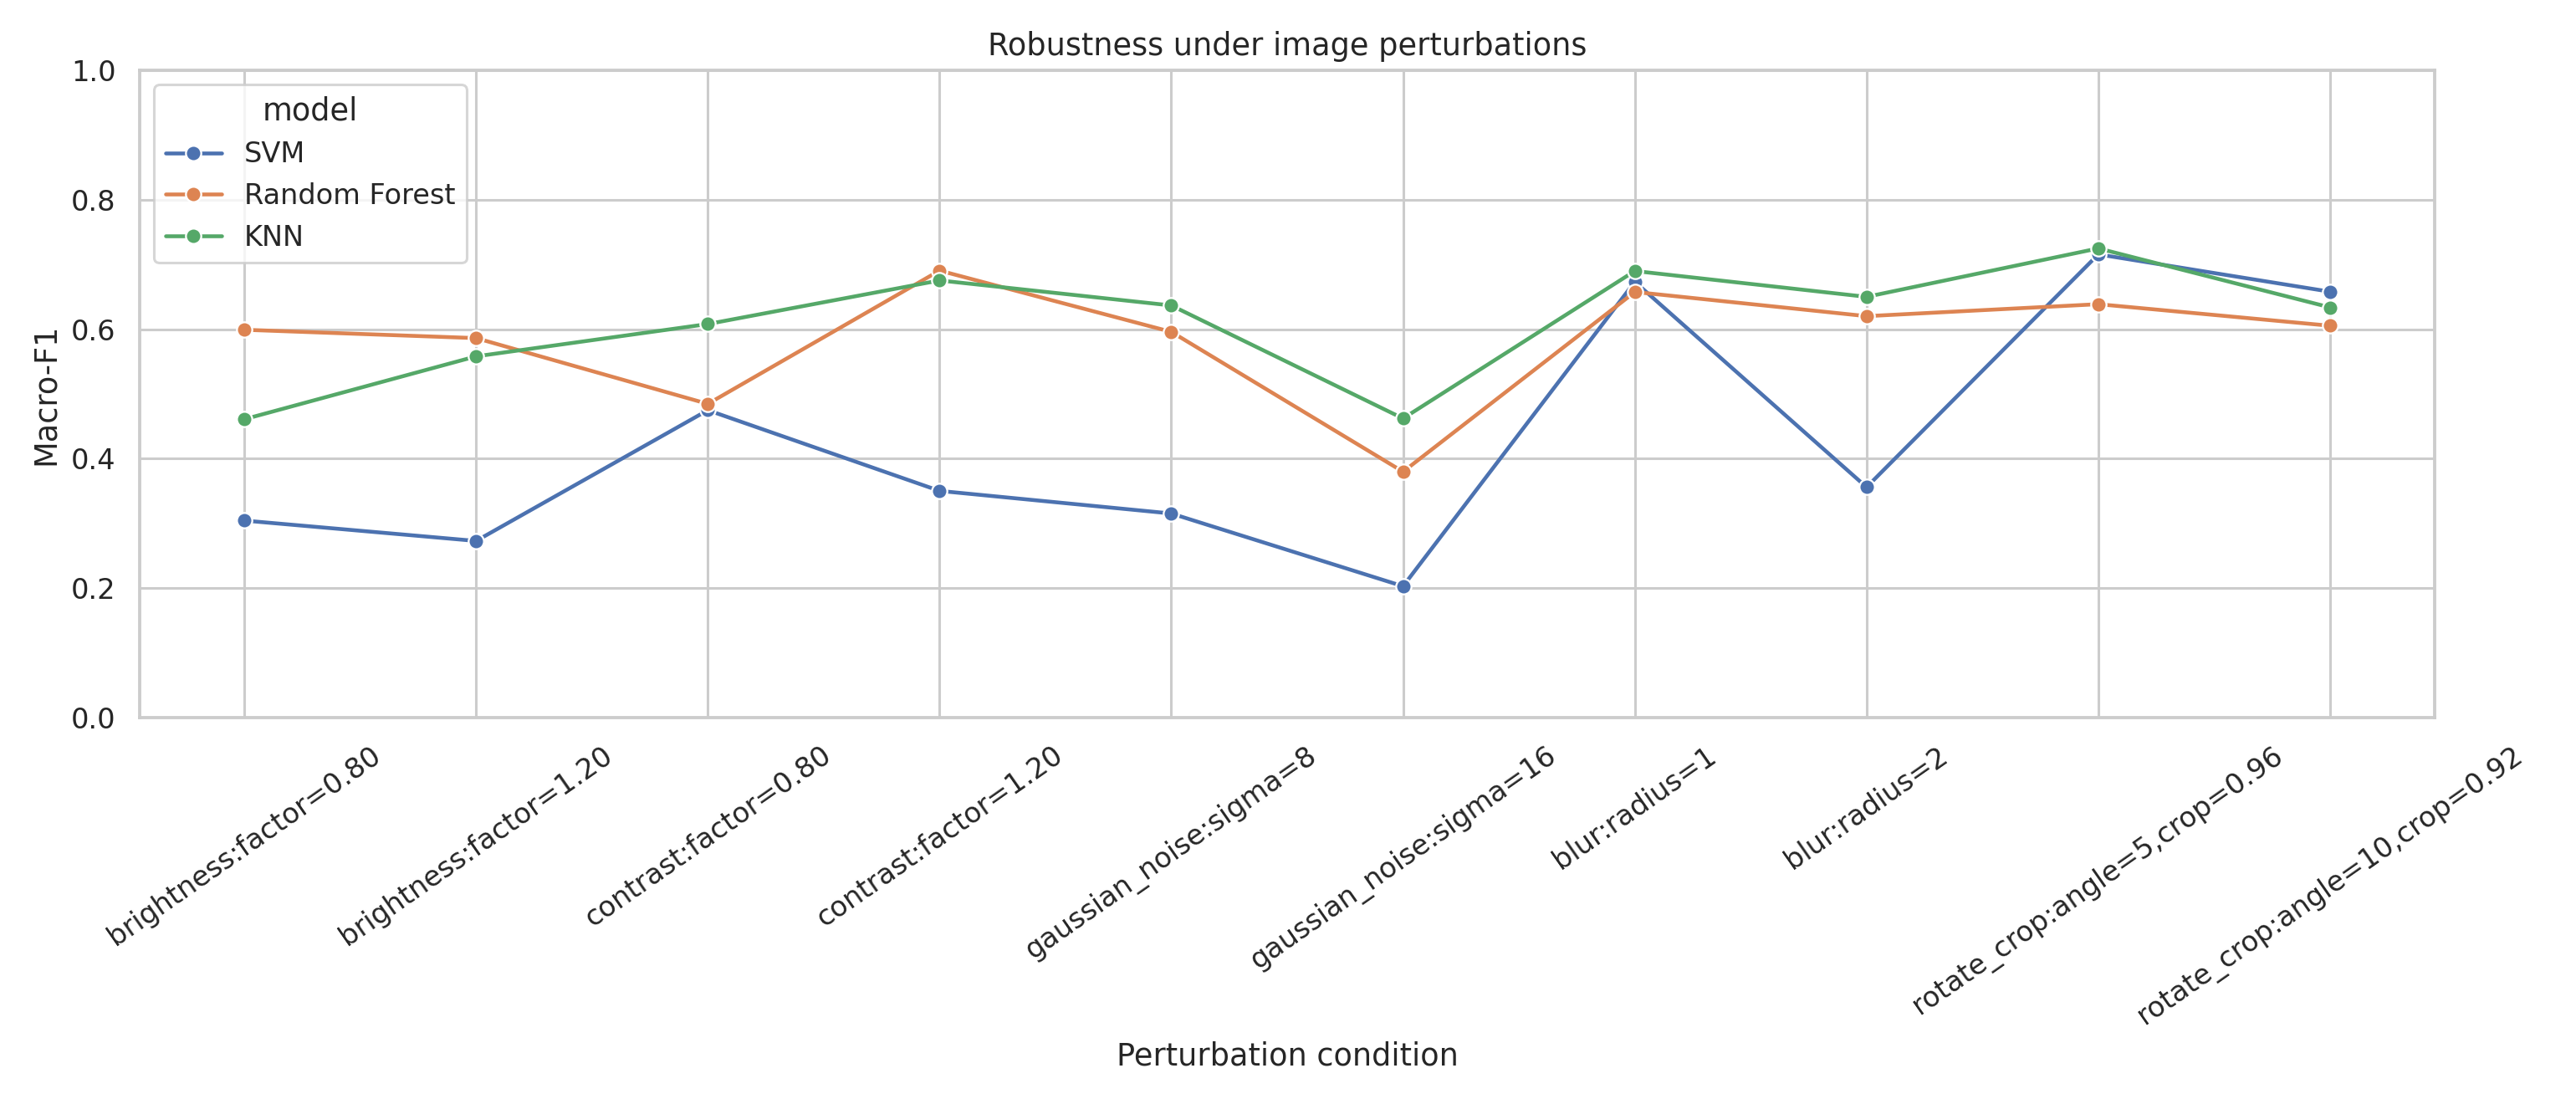
\includegraphics[width=0.95\textwidth]{./results_member4/robustness_curves.png}
\caption{不同扰动条件下三种模型的Macro-F1变化}
\label{fig:robust_curves}
\end{figure}

\begin{figure}[H]
\centering
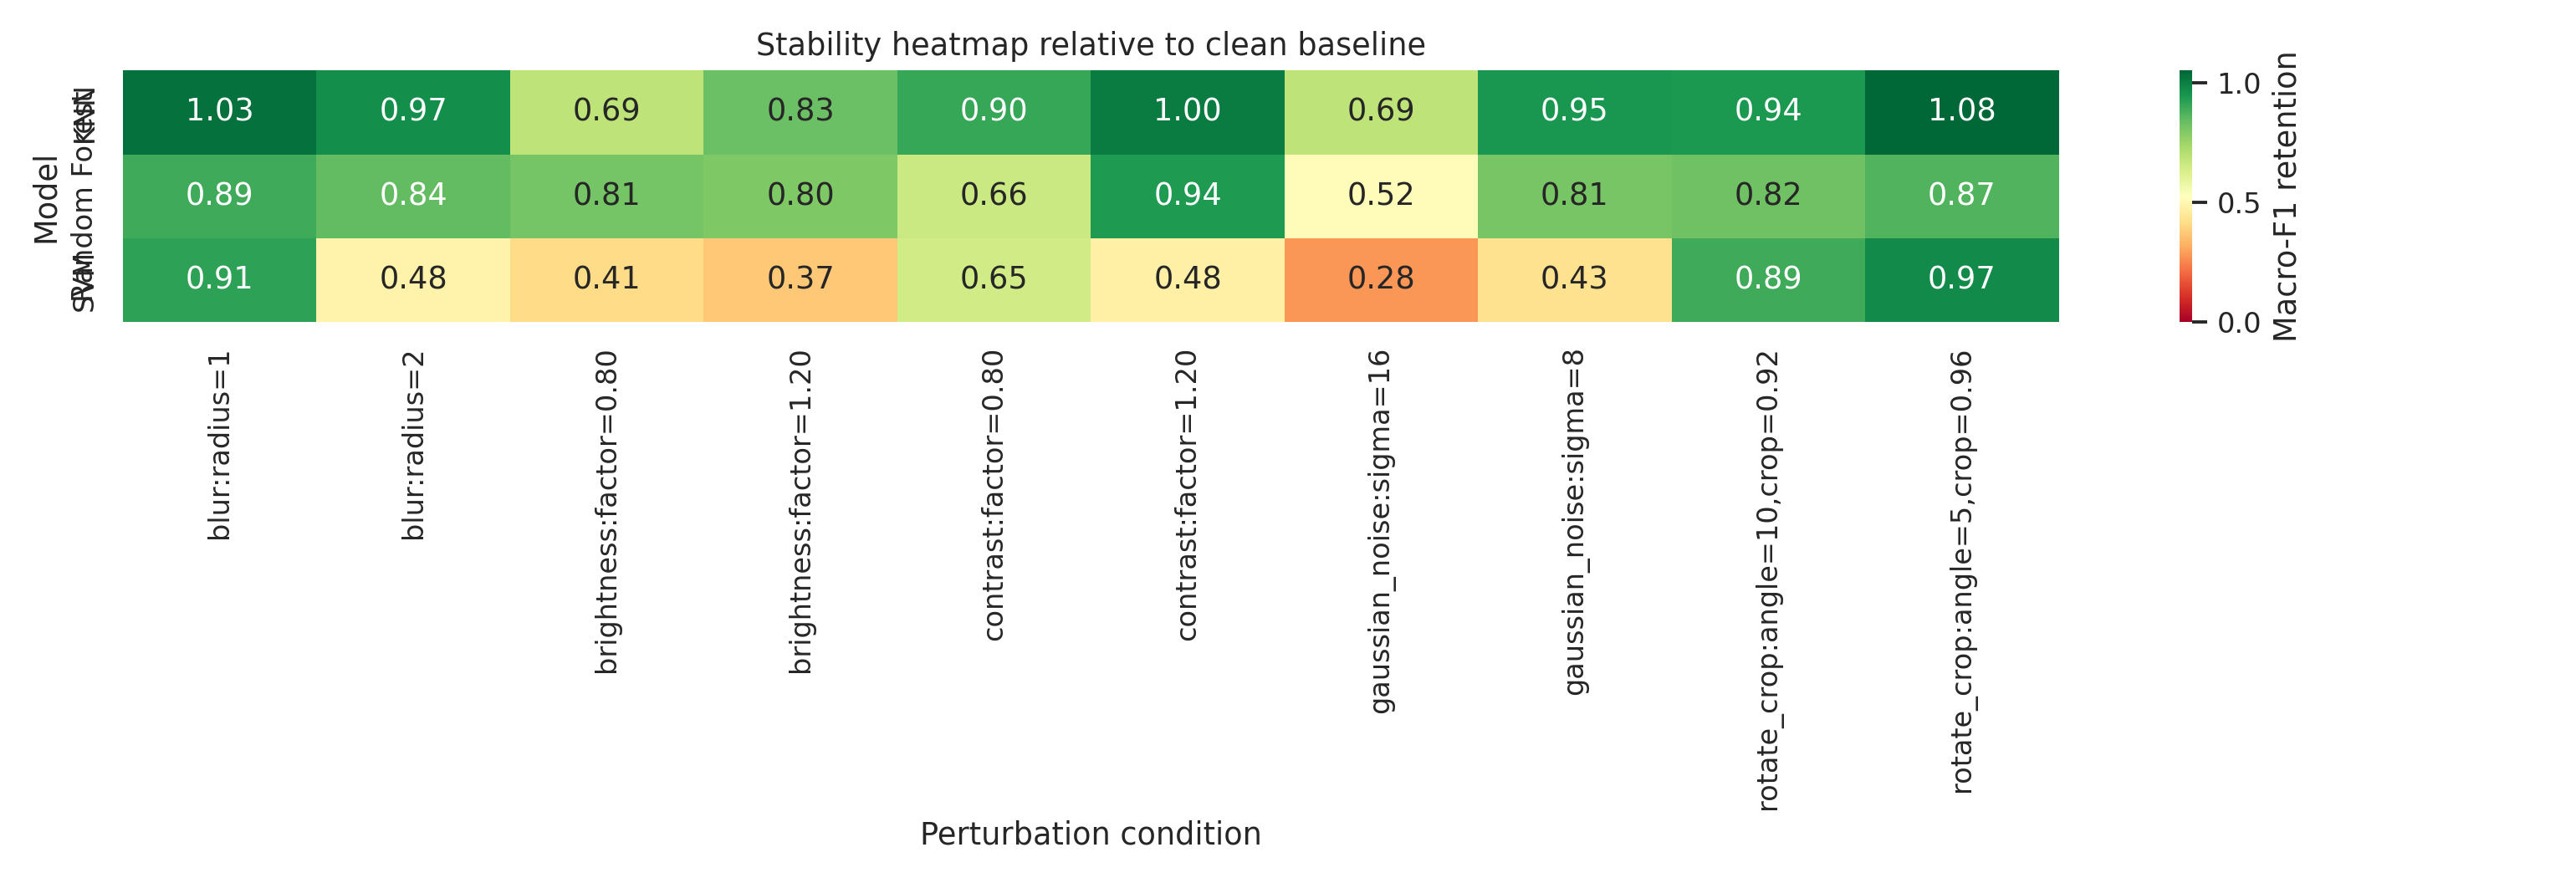
\includegraphics[width=0.95\textwidth]{./results_member4/stability_heatmap.png}
\caption{不同扰动条件下相对基线的Macro-F1保持率}
\label{fig:heatmap}
\end{figure}

\begin{table}[H]
\centering
\caption{各模型最差扰动条件}
\label{tab:worst_perturb}
\begin{tabular}{llllcc}
\toprule
\textbf{模型} & \textbf{最差扰动} & \textbf{强度} & \textbf{Accuracy} & \textbf{Macro-F1} & \textbf{F1保持率} \\
\midrule
SVM           & gaussian noise & $\sigma=16$ & 0.2500 & 0.2026 & 0.2752 \\
Random Forest & gaussian noise & $\sigma=16$ & 0.4333 & 0.3796 & 0.5158 \\
KNN           & brightness & factor=0.80 & 0.4417 & 0.4608 & 0.6856 \\
\bottomrule
\end{tabular}
\end{table}

由表\ref{tab:worst_perturb}可见，SVM在高斯噪声较强时下降最明显，Macro-F1仅保持基线的27.52\%。随机森林虽然也受高斯噪声影响，但F1保持率为51.58\%，明显高于SVM。KNN的最差扰动出现在亮度降低条件下，说明基于距离的模型对颜色直方图和颜色矩变化较敏感。

\begin{figure}[H]
\centering
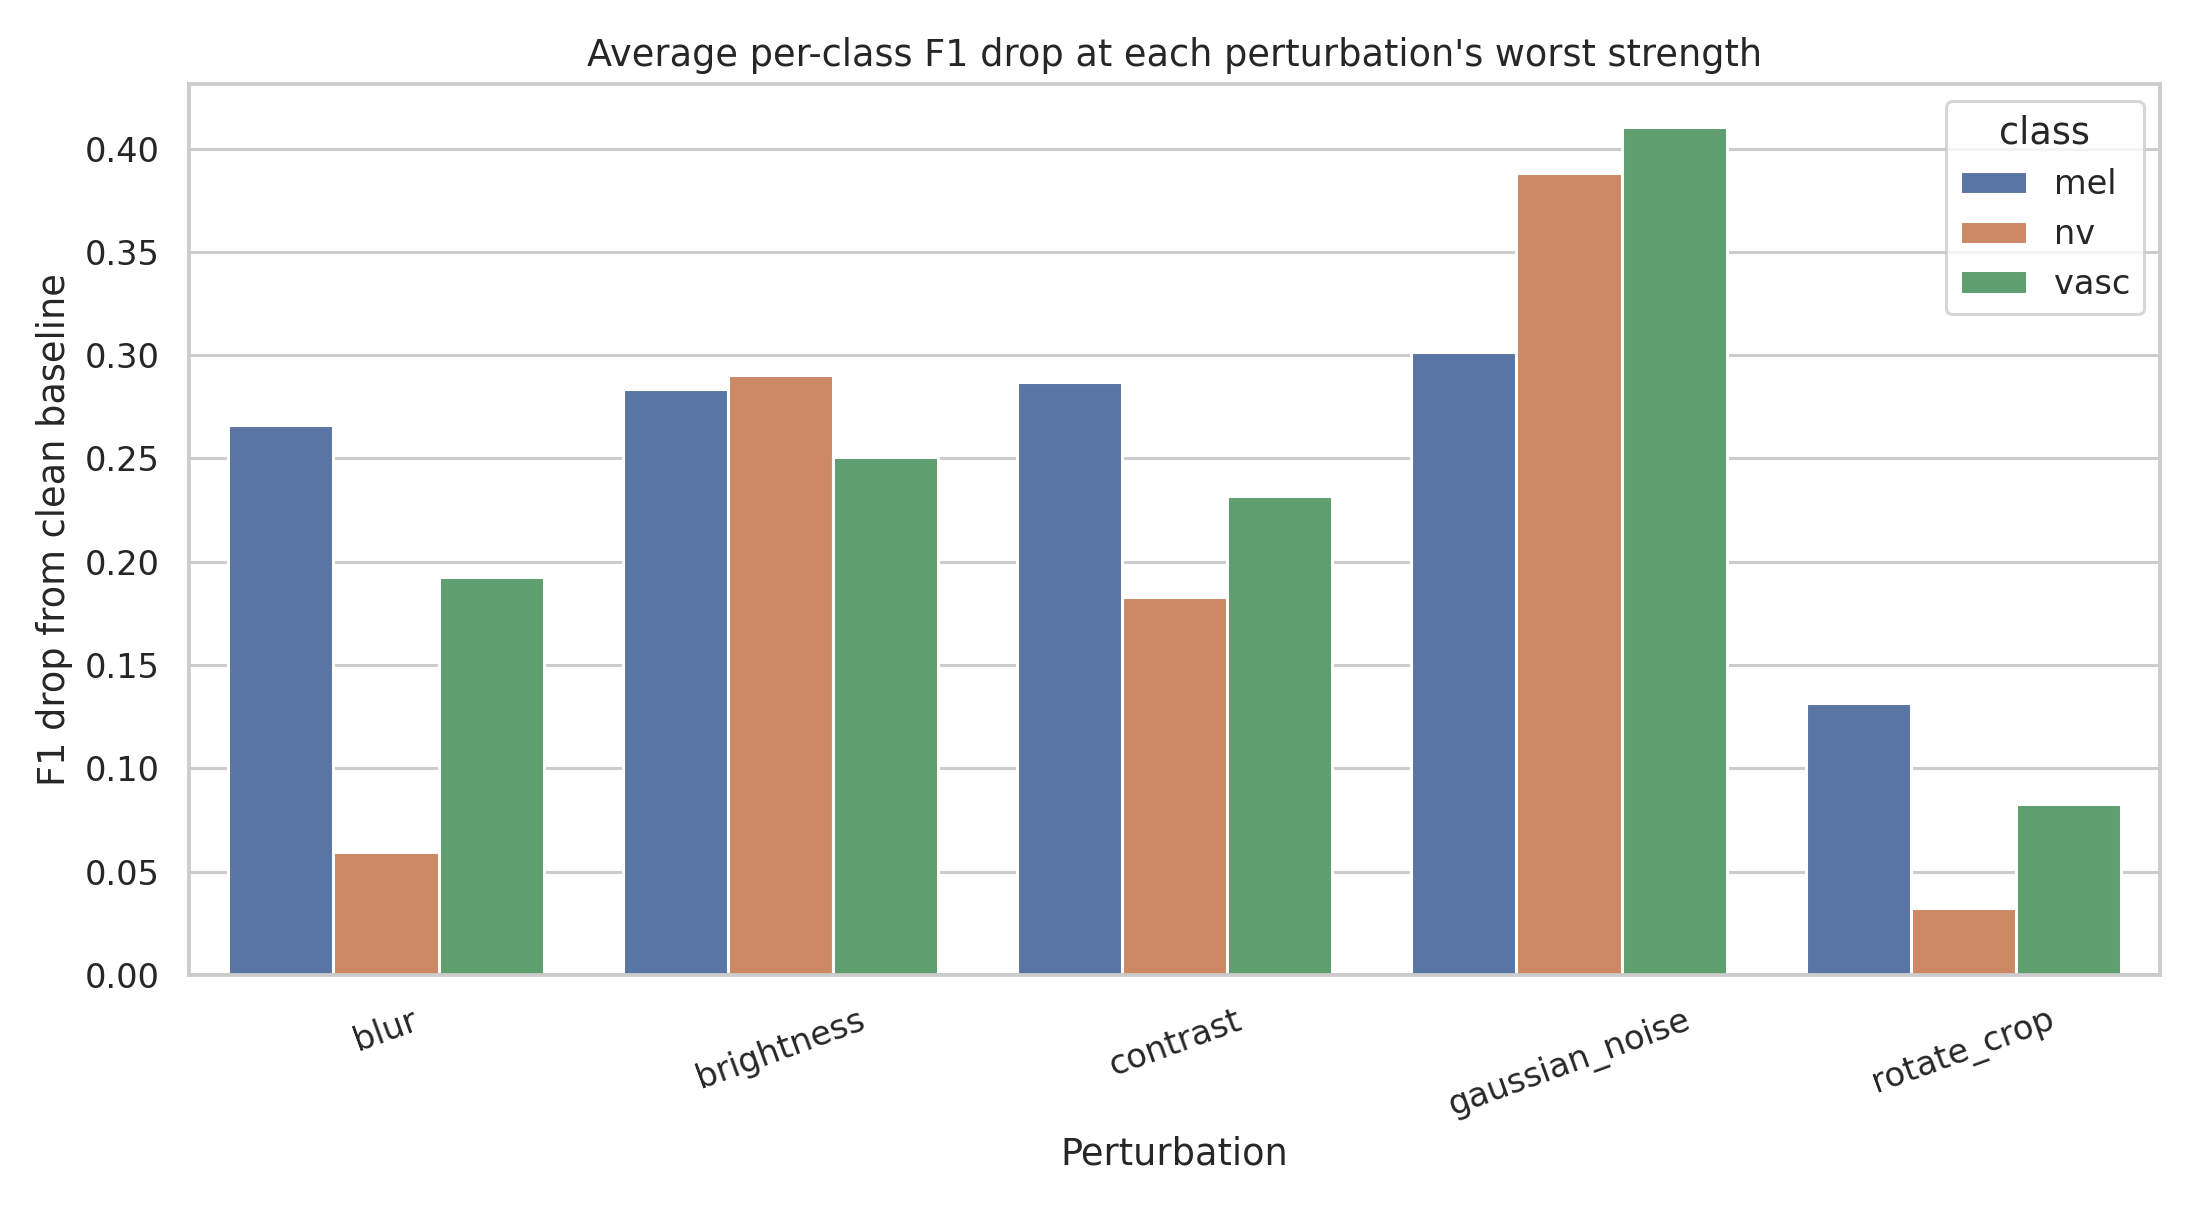
\includegraphics[width=0.82\textwidth]{./results_member4/per_class_f1_drop.png}
\caption{各类别在不同扰动下的F1下降}
\label{fig:per_class_drop}
\end{figure}

从图\ref{fig:per_class_drop}可以看到，mel和nv在多数扰动下的F1下降更明显，这与成员3报告中指出的 ``mel 与 nv 是主要混淆来源'' 一致。vasc虽然样本量较少，但颜色和纹理特征区分度较强，在部分扰动下相对更稳定。

\begin{figure}[H]
\centering
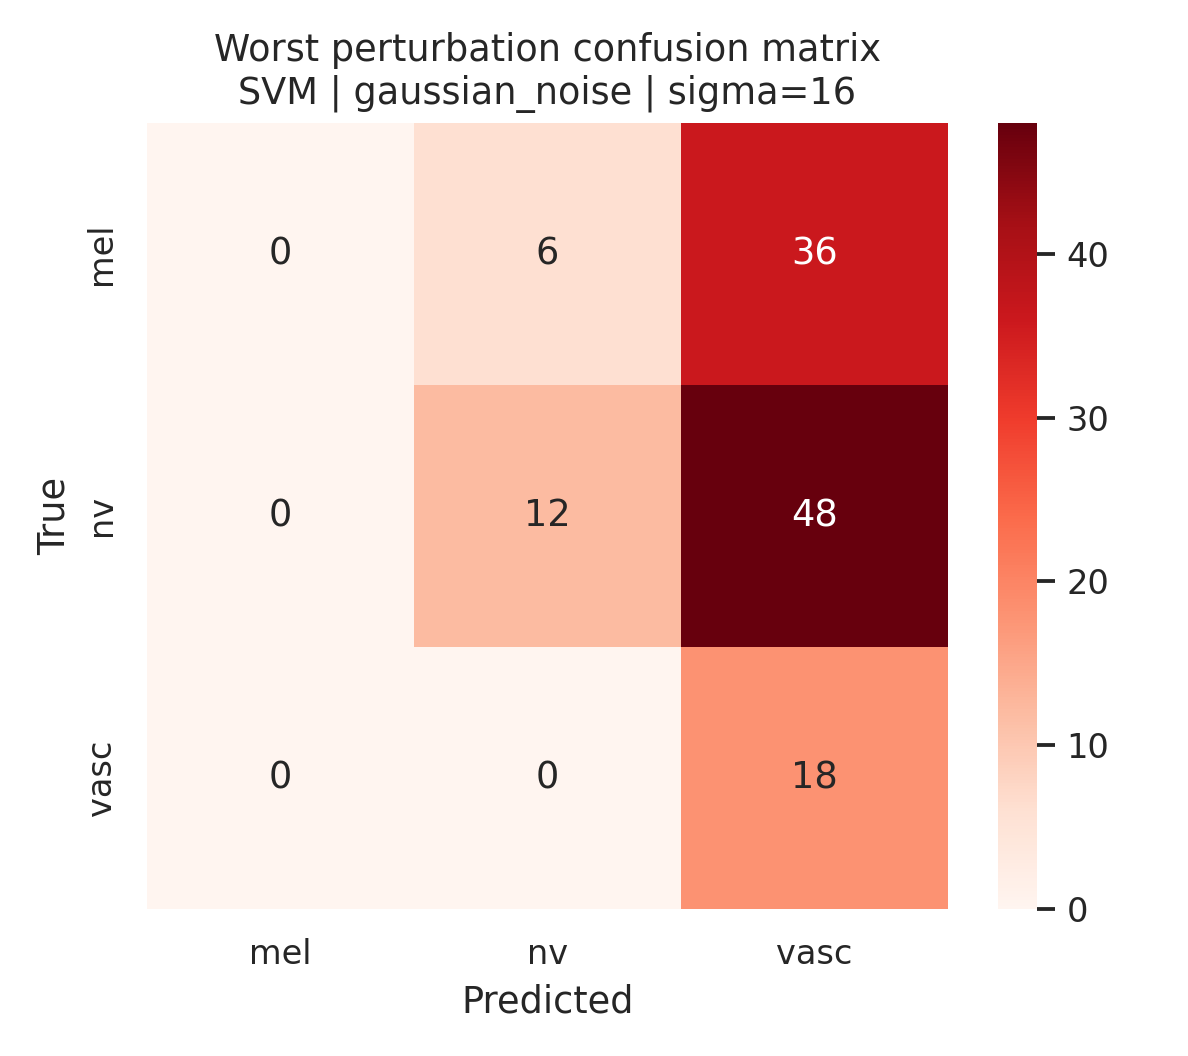
\includegraphics[width=0.60\textwidth]{./results_member4/worst_perturbation_confusion_matrix.png}
\caption{最差扰动条件下的混淆矩阵}
\label{fig:worst_cm}
\end{figure}

\subsection{严格分组稳定性分析}
为排除同源增强图像带来的评估偏差，本模块将同一原始编号的所有样本放在同一侧，进行10次严格分组随机划分。表\ref{tab:group_split}给出了均值和标准差。

\begin{table}[H]
\centering
\caption{严格分组划分下的稳定性结果}
\label{tab:group_split}
\begin{tabular}{lcccc}
\toprule
\textbf{模型} & \textbf{Accuracy} & \textbf{Accuracy std} & \textbf{Macro-F1} & \textbf{Macro-F1 std} \\
\midrule
SVM           & 0.5383 & 0.0500 & 0.5145 & 0.0496 \\
Random Forest & 0.6042 & 0.0320 & 0.5783 & 0.0346 \\
KNN           & 0.5158 & 0.0551 & 0.4903 & 0.0671 \\
\bottomrule
\end{tabular}
\end{table}

\begin{figure}[H]
\centering
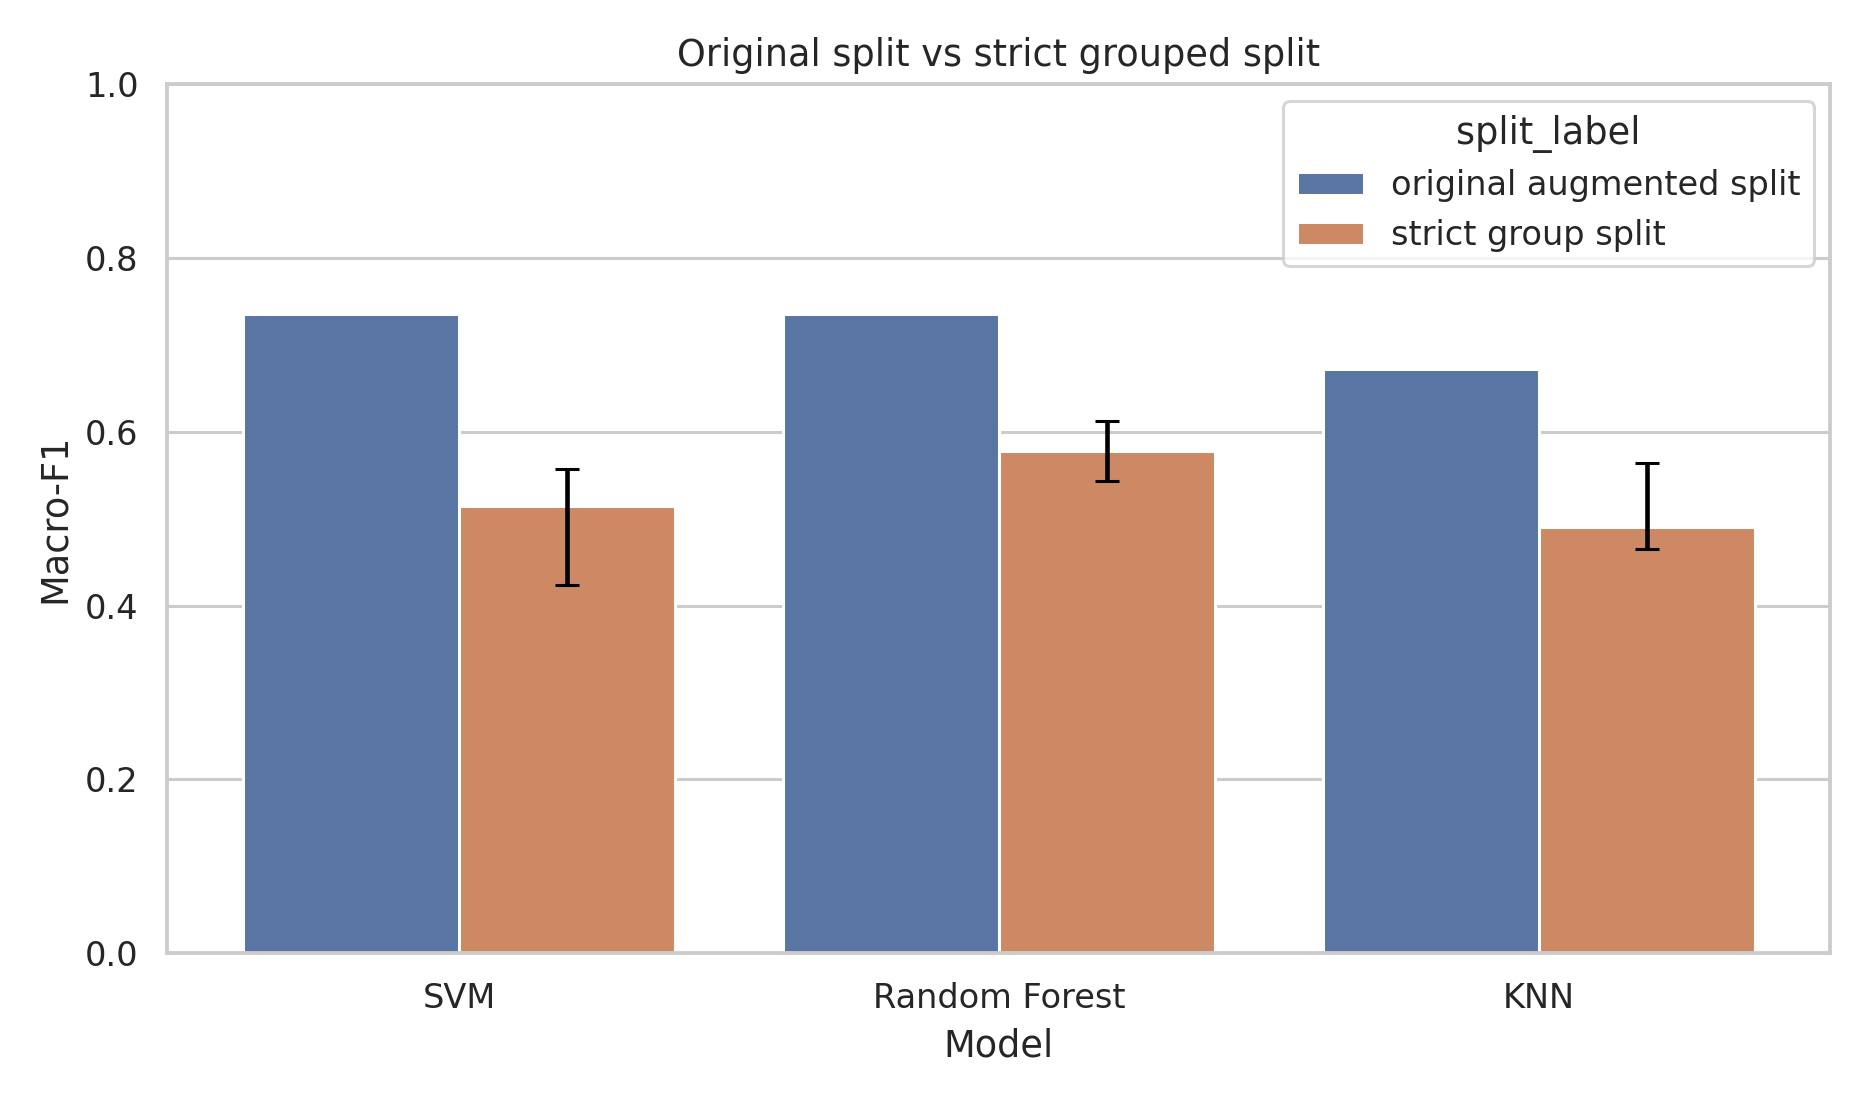
\includegraphics[width=0.82\textwidth]{./results_member4/group_split_stability.png}
\caption{原始增强样本划分与严格分组划分的Macro-F1对比}
\label{fig:group_split}
\end{figure}

严格分组后，三种模型性能均明显低于原始划分。其中随机森林仍保持最高的平均Macro-F1（0.5783），且标准差最小（0.0346），说明其对数据划分变化最稳定；SVM从原始划分的0.7360下降到0.5145，表明其在当前增强样本划分下可能受到了同源样本重叠的帮助；KNN均值最低且标准差最大，说明其泛化稳定性最弱。

\subsection{综合讨论}
\begin{enumerate}[label=(\arabic*)]
    \item \textbf{原始测试结果偏乐观}：训练集和测试集有98个原始编号重叠，这意味着基础测试集并非完全独立。严格分组后所有模型Macro-F1明显下降，说明同源增强图像会提高表面测试性能。
    \item \textbf{随机森林稳定性最好}：虽然随机森林在干净测试集上与SVM持平，但在严格分组和多数扰动条件下保持率更高，说明集成模型对特征扰动和划分变化更稳健。
    \item \textbf{SVM对强噪声敏感}：SVM在高斯噪声$\sigma=16$下Macro-F1降至0.2026，说明其决策边界对噪声导致的特征偏移较敏感。
    \item \textbf{KNN整体泛化能力较弱}：KNN在干净测试集、严格分组和增强一致性分析中均表现较弱，符合高维特征空间下距离度量退化的预期。
    \item \textbf{mel 与 nv 仍是主要难点}：扰动下各类别F1下降进一步说明，mel与nv的手工特征区分度不足，是后续深度学习或特征融合需要重点改进的方向。
\end{enumerate}

% ==================== 5. 总结 ====================
\section{总结}

本模块完成了传统机器学习模型的鲁棒性测试与稳定性分析，主要工作包括：
\begin{enumerate}[label=(\arabic*)]
    \item \textbf{基线复现}：复现成员3的SVM、随机森林和KNN测试集指标，确认后续分析基于同一性能起点；
    \item \textbf{增强一致性分析}：发现训练集与测试集存在98个原始编号重叠，并统计增强版本间预测一致性；
    \item \textbf{扰动鲁棒性测试}：对测试图像施加五类十组扰动，计算性能保持率、预测不变率和混淆矩阵；
    \item \textbf{严格分组测试}：按原始编号进行10次分组随机划分，检验模型在无同源样本泄漏条件下的真实稳定性；
    \item \textbf{可视化输出}：生成鲁棒性曲线、稳定性热力图、各类别F1下降图、严格分组对比图和最差扰动混淆矩阵。
\end{enumerate}

\textbf{最终结论：}
\begin{itemize}
    \item 若只看原始测试集，SVM和随机森林Macro-F1均约为0.7360，二者表现接近；
    \item 若考虑增强划分风险和严格分组泛化能力，随机森林更加稳定，Macro-F1为0.5783$\pm$0.0346；
    \item 当前增强数据划分存在同源样本重叠，最终报告中应明确说明该限制；
    \item 高斯噪声、亮度变化对传统手工特征模型影响显著，后续可通过更丰富的数据增强、颜色归一化或深度学习特征提升鲁棒性。
\end{itemize}

% ==================== 输出文件 ====================
\subsection{输出文件}

成员4代码与结果已保存如下：
\begin{itemize}
    \item \texttt{robustness\_analysis.py}：成员4鲁棒性分析主脚本；
    \item \texttt{results\_member4/robustness\_metrics.csv}：扰动条件下的完整指标表；
    \item \texttt{results\_member4/augmentation\_consistency.csv}：增强一致性与增强后缀子集性能；
    \item \texttt{results\_member4/group\_split\_comparison.csv}：原始划分与严格分组划分对比；
    \item \texttt{results\_member4/group\_split\_summary.csv}：严格分组10次实验均值与标准差；
    \item \texttt{results\_member4/robustness\_curves.png}：扰动鲁棒性曲线；
    \item \texttt{results\_member4/stability\_heatmap.png}：性能保持率热力图；
    \item \texttt{results\_member4/per\_class\_f1\_drop.png}：各类别F1下降图；
    \item \texttt{results\_member4/group\_split\_stability.png}：严格分组稳定性对比图；
    \item \texttt{results\_member4/worst\_perturbation\_confusion\_matrix.png}：最差扰动混淆矩阵；
    \item \texttt{report\_member4.tex / report\_member4.pdf}：成员4实验报告。
\end{itemize}

\end{document}
